\documentclass[border=5pt]{standalone}
\usepackage{fontspec,unicode-math}
\setmainfont{Noto Serif}
\setmathfont{STIXTwoMath-Regular.otf}
\usepackage{tikz}
\usetikzlibrary{arrows.meta,calc,patterns,decorations.markings,decorations.pathmorphing}
\tikzset{lev/.style={line width=1.25pt,line cap=butt},
 fine/.style={line width=.60pt},band/.style={line width=.57pt},
 curve/.style={line width=1.35pt,line cap=round,line join=round},
 ax/.style={line width=.65pt,-{Latex[length=2.3mm,width=1.3mm]}},
 ray/.style={line width=.68pt,-{Latex[length=2.0mm,width=1.10mm]}},
 dimension/.style={line width=.57pt,{Latex[length=1.7mm,width=.9mm]}-{Latex[length=1.7mm,width=.9mm]}},
 flow/.style={line width=.68pt,postaction={decorate},decoration={markings,mark=at position .66 with {\arrow{Latex[length=2mm,width=1.1mm]}}}},
 lab/.style={font=\fontsize{13}{16}\selectfont,inner sep=1.3pt},
 small/.style={font=\fontsize{11}{13}\selectfont,inner sep=1.2pt},
 tinytext/.style={font=\fontsize{10}{12}\selectfont,inner sep=1pt},
 panel/.style={font=\fontsize{14}{16}\selectfont\itshape,inner sep=0pt}}
\pagestyle{empty}
\begin{document}
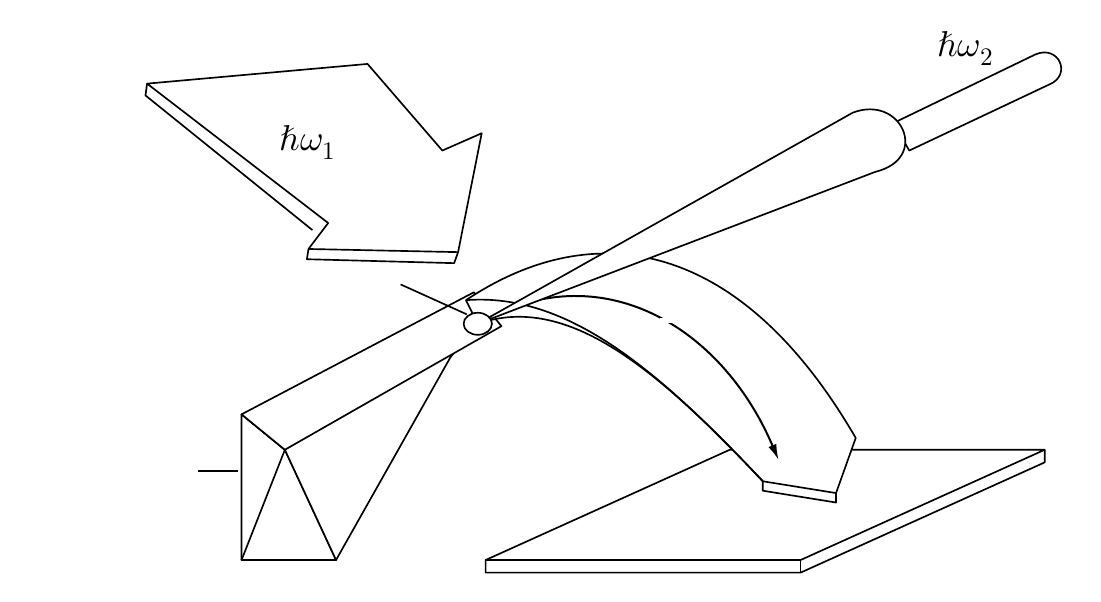
\begin{tikzpicture}[x=1cm,y=1cm,line join=round]
% Spatial arrangement is schematic; no optical element has been introduced.
\coordinate (Slot) at (2.65,1.55);\coordinate (I) at (5.1,3.15);\coordinate (Collect) at (9.05,1.23);
% Collector, drawn first, all faces share vertices.
\coordinate (CA) at (5.2,.15);\coordinate (CB) at (9.2,.15);\coordinate (CC) at (12.3,1.55);\coordinate (CD) at (8.3,1.55);
\path[draw,fine,fill=white] (CA)--(CB)--(CC)--(CD)--cycle;
\draw[fine] (CA)--++(0,-.16)--($(CB)+(0,-.16)$)--($(CC)+(0,-.16)$)--(CC);
\draw[fine] (CB)--++(0,-.16);
\node[lab,rotate=0] at (8.4,.63) {Коллектор};
% Slot source with two walls and a narrow aperture.
\path[draw,fine,fill=white] (2.1,.15)--(2.1,2.0)--(Slot)--(3.3,.15)--cycle;
\path[draw,fine,fill=white] (Slot)--(3.25,2.2)--(5.08,3.15)--(4.75,2.72)--(3.3,.15)--cycle;
\draw[fine] (2.1,.15)--(Slot)--(2.1,2.0);
% Atomic-vapor sheet reaching the interaction region.
\path[draw,fine,fill=white] (2.1,2.0)--(5.05,3.55)--(5.4,3.12)--(Slot)--cycle;
% Ion ribbon, all boundaries tied to the interaction and collector.
\path[draw,fine,fill=white] (4.95,3.45) .. controls (6.6,4.55) and (8.45,4.2) .. (9.90,1.7)
 --(9.65,1.00)--(8.72,1.15) .. controls (7.4,2.55) and (6.25,3.55) .. (5.1,3.15)--cycle;
\draw[fine] (4.95,3.45) .. controls (6.25,3.55) and (7.4,2.55) .. (8.72,1.15);
\draw[fine] (8.72,1.15)--++(0,-.12)--(9.65,.88)--(9.65,1.0);
% Ion extraction direction is a curve whose origin is the shared interaction I;
% its end lies on the collector, not at a free page coordinate.
\draw[ray,line width=.72pt] (I) .. controls (6.65,4.05) and (8.20,3.12) .. (8.92,1.42);
\node[lab,fill=white,inner sep=1pt] at (7.70,3.19) {Ионы};
% Hollow pump arrow.
\coordinate (PumpTip) at (4.85,4.06);
\path[draw,fine,fill=white] (.9,6.2)--(3.7,6.45)--(4.65,5.35)--(5.15,5.57)--(PumpTip)--(2.95,4.10)--(3.2,4.43)--cycle;
\draw[fine] (.9,6.2)--(.88,6.05)--(3.0,4.34) (2.95,4.10)--(2.93,3.97)--(4.80,3.92)--(PumpTip);
\node[lab] at (2.95,5.45) {$\hbar\omega_1$};
% Ionizing beam: barrel and conical arrow, aimed at the same interaction region.
\path[draw,fine,fill=white] (10.38,5.7)--(12.18,6.57) .. controls (12.48,6.7) and (12.65,6.31) .. (12.36,6.19)--(10.58,5.35)--cycle;
\path[draw,fine,fill=white] (I)--(9.86,5.83) .. controls (10.48,6.07) and (10.85,5.25) .. (10.15,5.08)--cycle;
\node[lab] at (11.3,6.65) {$\hbar\omega_2$};
% Interaction cross-section and labels are last, not painted behind ribbons.
\draw[fine,fill=white] (I) ellipse (.18 and .14);
\node[lab,anchor=east] (Vapor) at (4.12,3.65) {Облучаемый пар};
\draw[fine] (Vapor.east)--($(I)+(-.14,.12)$);
\node[lab,align=left,anchor=east] (Source) at (1.55,1.28) {Щелевой источник\\атомного пара};
\draw[fine] (Source.east)--(2.05,1.28);

\end{tikzpicture}
\end{document}
